\documentclass{article}
\usepackage[left=2cm,right=2cm,top=2cm,bottom=2cm]{geometry}
\usepackage[utf8]{inputenc}
\usepackage[german]{babel}
\usepackage{amsmath}
\usepackage{dsfont}
\usepackage[export]{adjustbox}
\usepackage{amsthm}
\usepackage{color}
\usepackage{amsfonts}
\usepackage{amssymb}
\usepackage{wasysym}
\usepackage{makeidx}
\usepackage{graphicx}
\usepackage[colorlinks=true,urlcolor=blue,linkcolor=blue]{hyperref}
\usepackage{ziffer}
\usepackage{minted}
\usepackage{xcolor}
\usepackage{framed}
\usepackage{mdframed}
\usepackage{subfiles}
\usemintedstyle{emacs}

\definecolor{purp}{HTML}{9A72AC}
\definecolor{re}{HTML}{FC6255}
\definecolor{gre}{HTML}{83C167}
\definecolor{blu}{HTML}{58C4DD}
\definecolor{shadecolor}{rgb}{0.85,0.85,0.85}
\definecolor{bg}{rgb}{0.95,0.95,0.95}
\setlength{\parindent}{0em} 

\BeforeBeginEnvironment{minted}{\begin{mdframed}[linewidth =2 ,backgroundcolor=bg , linecolor=black, linewidth=0.5]}
\AfterEndEnvironment{minted}{\end{mdframed}}

\newtheorem{defi}{Definition}
\BeforeBeginEnvironment{defi}{\begin{mdframed}[linewidth =2 ,backgroundcolor=bg , linecolor=black, linewidth=0.5]}
\AfterEndEnvironment{defi}{\end{mdframed}}

\newcommand{\bsp}{\textbf{Beispiel}:}
%\newcommand{\task}{\textbf{Aufgabe}:}

\newcommand{\bol}[1]{\textbf{#1}}
\newcommand{\q}[1]{\glqq #1\grqq}
\newcommand{\DODO}[1]{\textbf{\textcolor{red}{DODO:}} #1 \\ \begin{center}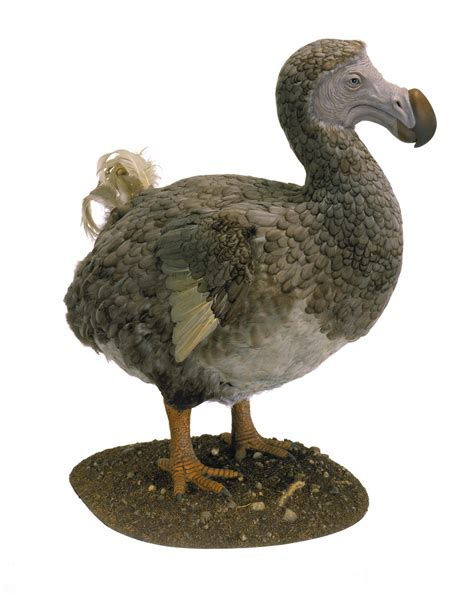
\includegraphics[scale=0.2]{../../media/dodo.jpg} \end{center}}

\newenvironment{task}[1]{
    \begin{shaded*}
    \textbf{Aufgabe #1}:
}{
    \end{shaded*}
}

\begin{document}
Übersetzungen aller Code-Schnipsel im Text:
Code-Fragment 1:
\begin{minted}{Java}
    int[] feld = new int[5];
\end{minted}
Code-Fragment 2:
\begin{minted}{Java}
    Mensch[] menschen = new Mensch[5]:
\end{minted}
Code-Fragment 3:
\begin{minted}{Java}
    int[] zahlen = {5,3,42,17,-2};
    int dritterEintrag = numbers[2];
    System.out.println(dritterEintrag);
\end{minted}
Code-Fragment 4 - erste Definition der Klasse Mensch:
\begin{minted}{Java}
    public class Mensch() {
        private String name;
        private int alter; 
    
        public Human(String name, int alter){
            this.name = name;
            this.alter = alter;
        }
    
    }
\end{minted}
Code-Fragment 5 - erste Definition der Klasse MeineListeFeld:
\begin{minted}{Java}
    public class MeineListeFeld(){

        private Mensch[] warteschlange;
        private int anzahl;

        public MeineListeFeld() {
            warteschlange = new Mensch[5];
            anzahl = 0;
        }

    }
\end{minted}
Code-Fragment 6:
\begin{minted}{Java}
    public void hintenAnfügen(Mensch mensch) 
\end{minted}
Code-Fragment 7 - erste Implementierung von hintenAnfügen:
\begin{minted}{Java}
    public void hintenAnfügen(Mensch mensch) {
        for(int i = 0; i < warteschlange.length; i++) {
            if(warteschlange[i] == null) {
                warteschlange[i] = mensch;
            }
        }
    }
\end{minted}
Code-Fragment 8 - zweite Version von hintenAnfügen:
\begin{minted}{Java}
    public class MeineListeFeld(){

        private Mensch[] warteschlange;
        private int anzahl; 

        public MeineListeArray() {
            warteschlange = new Mensch[5];
            anzahl = 0;
        }

        public void hintenAnfügen(Mensch mensch) {
            warteschlange[anzahl] = mensch;
            anzahl++;
        }

    }
\end{minted}
Code-Fragment 9 - finale Version von hintenAnfügen: 

\begin{minted}{Java}
    public void hintenAnfügen(Mensch mensch) {
        if(anzahl == warteschlange.length) {
            warteschlangeVergroessern();
        } 
        warteschlange[anzahl] = mensch;
        anzahl++;
    }

    private void warteschlangeVergroessern() {
        Mensch[] neueWarteschlange = new Mensch[warteschlange.length + 10];
        for(int i = 0; i < warteschlange.length; i++){
            neueWarteschlange[i] = warteschlange[i];
        }
        warteschlange = neueWarteschlange;
    }
\end{minted}
Code-Fragment 10 - Implementierung von vorneEntfernen:
\begin{minted}{Java}
    public Mensch vorneEntfernen() {
        if(warteschlange[0] == null) {
            return null;
        }
        Mensch zuEntfernen = warteschlange[0];
        for(int i = 0; i < warteschlange.length -1; i++){
            if (warteschlange[i+1] == null){
                break;
            }
            warteschlange[i] = warteschlange[i+1];
        }
        warteschlange[warteschlange.length-1] = null;
        anzahl--;
        return zuEntfernen;    
    }
\end{minted}
\end{document}